\documentclass[12pt,twoside,final]{book}

%%%%%%%%%
% My packages
%%%%%%%%
\usepackage{rotating}
%%%%%%%%%
% My packages
%%%%%%%%


\usepackage[portuges,brazil]{babel}
\usepackage[latin1]{inputenc}
\usepackage{indentfirst}
\usepackage{ae}
\usepackage{harvard}
\usepackage{amssymb,fancyhdr,fancybox,epsfig,psfrag,amsmath,tabularx}
\usepackage[paperwidth=8.5in,paperheight=11in,hmargin={25mm,20mm},vmargin={20mm,20mm}]{geometry} %tamanho letter



\usepackage[color]{showkeys}
\definecolor{refkey}{rgb}{0.39,0.58,1}
\definecolor{labeled}{rgb}{1,0,0}
\usepackage[Lenny]{fncychap}
\setlength{\headheight}{15pt}

%=========================================== Headers =========================================

\renewcommand{\chaptermark}[1]{\markboth{\chaptername\ \thechapter. \ #1}{ }}
\renewcommand{\sectionmark}[1]{\markright{\thesection. \ #1}}
\fancyhead{}
\fancyfoot{}
\fancyhead[LE,RO]{\thepage}
\fancyhead[RE]{\nouppercase{\leftmark}}
\fancyhead[LO]{\nouppercase{\rightmark}}
%==============================================================================================


% Espacos H2, Hoo, L2, Loo
\newcommand\Hi{{\mathcal{H}}_{\infty}}
\newcommand\Hd{{\mathcal{H}}_{2}}
\newcommand\Li{{\mathcal{L}}_{\infty}}
\newcommand\Ld{{\mathcal{L}}_{2}}


\def\reais{{\rm I\kern-.17em R}} % R de reais
\def\Dest{{\rm I\kern-.17em D}} % R de reais
\newcommand{\Dgest}{\ensuremath{\mathcal{D}}}
\newcommand{\naturais}{\mathbb{N}}
\newcommand{\inteiros}{\mathbb{Z}_{+}}
\newcommand{\matlab}{{\sc Matlab}}

%super parenteses
\makeatletter
\def\Biggg#1{{\hbox{$\left#1\vbox to29\p@{}\right.\n@space$}}}
\newdimen\bracketwidth
\settowidth{\bracketwidth}{\Biggg(} \makeatother


%\newcommand{\carinha}{\raisebox{-.2ex}{\epsfxsize 3mm \epsffile{cara.eps}}}

% Bolds
\newcommand{\I}{{\bf I}}
\newcommand{\Z}{{\bf 0}}
\newcommand{\Bfres}{\mathcal{B}}

% funcoes
\newcommand{\Tr}{\mbox{Tr}}

% Referencia com parenteses
\newcommand{\bref}[1]{\mbox{(\ref{#1})}}

% Ambiente de equacoes
\newcommand\be{\begin{equation}}
\newcommand\ee{\end{equation}}
\newcommand\vi{\vspace{\baselineskip}}

% newtheorems e similares

\newtheorem{teorema}{\noindent{\bf Teorema} }[chapter]
\newtheorem{lema}{\noindent{\bf Lema} }[chapter]
\newtheorem{corolario}{\noindent{\bf Corol�rio} }[chapter]
\newenvironment{prova}{\noindent{\bf Prova:}}{\null\hfill $\rule{1.5mm}{1.5mm}$}
\newtheorem{definicao}{\noindent{\bf Defini��o} }[chapter]

\newcommand{\simplex}{\Delta_N}



\newcommand{\Aal}{A(\alpha)}
\newcommand{\Bal}{B(\alpha)}
\newcommand{\Cal}{C(\alpha)}
\newcommand{\Dal}{D(\alpha)}


\newcommand{\Pal}{P(\alpha)}
\newcommand{\Gal}{G(\alpha)}
\newcommand{\Hal}{H(\alpha)}
\newcommand{\Qal}{Q(\alpha)}
\newcommand{\Xal}{X(\alpha)}
\newcommand{\Xual}{X_1(\alpha)}
\newcommand{\Xdal}{X_2(\alpha)}

\newcommand{\Sfr}{\mathcal{S}}

\newcommand{\Xfal}{\mathcal{X}(\alpha)}
\newcommand{\Bfal}{\mathcal{B}(\alpha)}
\newcommand{\Qfal}{\mathcal{Q}(\alpha)}
\newcommand{\Sfal}{\mathcal{S}(\alpha)}

\newcommand{\Kfr}{\mathcal{K}}
\newcommand{\Ifr}{\mathcal{I}}
\newcommand{\Afr}{\mathcal{A}}
\newcommand{\Pfr}{\mathcal{P}}
\newcommand{\Cfr}{\mathcal{C}}
\newcommand{\Gfr}{\mathcal{G}}


\begin{document}

%\pagenumbering{roman}
\pagestyle{plain}

%Tese em portugu�s
%================================================================================================
%================================= PRIMEIRA FOLHA INTERNA  ======================================
%================================================================================================

\thispagestyle{empty} %Tirando o numero da primeira p�gina
\vspace*{2.0cm}
\begin{center}
\large Tiago de Freitas Pereira
\end{center}

\vspace*{6.8cm}

\begin{center}
{\sc A Comparative Study of Countermeasures to Detect Spoofing Attacks in Face Authentication Systems}
\end{center}

\vspace*{3.25cm}


\null \vfill

\begin{center}
Campinas\\2013
\end{center}
\newpage
% parte de tr�s da primeira folha interna fica em branco

\null \vfill
\newpage

%================================================================================================
%====================================== FOLHA DE ROSTO ==========================================
%================================================================================================
\begin{center}
\large Universidade Estadual de Campinas\\
Faculdade de Engenharia El�trica e de Computa��o
\end{center}

\vspace*{1.5cm}
\begin{center}
\large Tiago de Freitas Pereira
\end{center}


\vspace*{2.3cm}

\begin{center}
{\sc A Comparative Study of Countermeasures to Detect Spoofing Attacks in Face Authentication Systems}

\end{center}

\vspace*{3.0cm}

\begin{flushright}
\begin{minipage}{9.0cm}
Disserta��o de Mestrado apresentada na Faculdade de Engenharia El�trica e de Computa��o como  parte dos
requisitos exigidos para a obten��o do t�tulo de Mestre em Engenharia El�trica. �rea de
concentra��o: Computa��o

\vspace*{0.5cm}
Orientador: Professor Doutor Jos� Mario De Martino

\end{minipage}
\end{flushright}

\null \vfill
\begin{minipage}{7cm}
\small
Este exemplar corresponde a vers�o final da disserta��o de mestrado apresentado pelo
aluno, e orientado pelo Prof. Dr. Jos� Mario De Martino\\[4mm]
\rule{7.0cm}{0.2mm} \hfill
\end{minipage}

\vspace*{0.5cm}

\begin{center}
Campinas\\2013
\end{center}

\newpage
\null \vfill
\newpage

%Tese em portugu�s e ingl�s
%%================================================================================================
%================================= PRIMEIRA FOLHA INTERNA  ======================================
%================================================================================================
\vspace*{2.0cm}
\begin{center}
\large Fulano de Tal
\end{center}


\vspace*{4.8cm}

\begin{center}
{\sc \Large  Coloque aqui o t�tulo da tese; Coloque aqui o t�tulo \\ da tese;
Coloque aqui o t�tulo da tese;  Coloque aqui }
\end{center}

\vspace*{1cm}
\begin{center}
{\sc \Large  Place here the thesis' title;Place here the thesis'\\ title; Place here the thesis' title ;
Place here }
\end{center}

\vspace*{3.25cm}


\null \vfill

\begin{center}
Campinas\\2012
\end{center}
\newpage
% parte de tr�s da primeira folha interna fica em branco

\null \vfill
\newpage


%================================================================================================
%====================================== FOLHA DE ROSTO ==========================================
%================================================================================================

\begin{center}
\large Universidade Estadual de Campinas\\
Faculdade de Engenharia El�trica e de Computa��o
\end{center}

\vspace*{1.0cm}
\begin{center}
\large Fulano de Tal
\end{center}


\vspace*{1.3cm}

\begin{center}
{\sc  Coloque aqui o t�tulo da tese; Coloque aqui o t�tulo da tese;  \\ 
Coloque aqui o t�tulo da tese;  Coloque aqui o t�tulo da tese;}
\end{center}

\vspace*{0.5cm}

\begin{center}
{\sc   Place here the thesis' title;Place here the thesis'\\ title; Place here the thesis' title ;
Place here }
\end{center}

\vspace*{1.0cm}

\begin{flushright}
\begin{minipage}{11.0cm}
Tese de doutorado apresentada � Faculdade de Engenharia El�trica e de Computa��o como  parte dos
requisitos exigidos para a obten��o do t�tulo de Doutor em Engenharia El�trica. �rea de
concentra��o: Automa��o. 

\vspace*{0.5cm}

Doctorate thesis presented to the School of Electrical and Computer Engineering
in partial fulfillment of the requirements for the degree of Doctor in Electrical
Engineering. Concentration area: Automation

\vspace*{1.0cm}
Orientador (Tutor): Prof. Dr. Pedro Luis Dias Peres

\end{minipage}
\end{flushright}

\null \vfill
\begin{minipage}{7cm}
\small
Este exemplar corresponde � vers�o final da tese defendida pelo
aluno, e orientada pelo Prof. Dr. Pedro Luis Dias Peres\\[4mm]
\rule{7.0cm}{0.2mm} \hfill 
\end{minipage}

\begin{center}
Campinas\\2012
\end{center}

%================================================================================================
%============================== Ficha (Somente na vers�o final) =================================
%================================================================================================
\newpage

\begin{center}
\vspace*{10cm}
Insira nesta p�gina a sua ficha catalogr�fica (somente vers�o final). Obs. � conveniente
converter o documento fornecido pela BAE (normalmente .doc) em um arquivo .ps. Para a vers�o
preliminar da tese (antes da defesa), simplesmente remova essa p�gina.
\end{center}
% Observa��o: a ficha fornecida pela BAE normalmente � fornecida em formato .doc. Existem diversas
% maneiras de converter .doc em .ps. 

% Descomente as duas pr�ximas linhas (e comente acima desde o begin{center} at� o end{center}) para inserir a ficha catalogr�fica caso a mesma j�  tenha sido convertida para .ps (no caso ficha.ps)

%\epsfxsize=0.925\columnwidth
%\epsffile{ficha.ps}

\null \vfill
\newpage

%================================================================================================
%============================== Folha de aprova��o (Somente na vers�o final) ====================
%================================================================================================


\begin{center}
\vspace*{10cm}
Insira nesta p�gina a folha de aprova��o fornecida pelo seu programa de p�s-gradua��o (somente vers�o final). 
Obs. � conveniente scanear o documento e convert�-lo para o formato .ps. Para a vers�o
preliminar da tese (antes da defesa), simplesmente remova essa p�gina.
\end{center}

% Escanear a folha de aprova��o fornecida pela CPG e converter para .ps ou .eps. A id�ia
% � inserir como uma figura. � muito prov�vel que ser� necess�rio fazer ajustes no
% tamanho, mexendo no comando \epsfxsize

% Descomente as duas pr�ximas linhas (e comente acima desde o \begin{center} at� o \end{center})
%\epsfxsize=0.985\columnwidth
%\hspace*{-1.25cm}\epsffile{aprov.eps}

\null \vfill
\newpage
% verso da folha de aprova��o em branco
\null \vfill
\newpage


%%======================================== Dedicat�ria =========================================
\null\vfill
\begin{flushright}
\begin{minipage}{6.5cm}
{\sc Dedicat�ria}
\end{minipage} \\[8mm]
\end{flushright}
\newpage %verso em branco

\null
%==============================================================================================


%%======================================= Agradecimentos =======================================
\chapter*{Agradecimentos}


\noindent Agrade�o,\\[2mm]

\newpage %verso em branco

\null

%==============================================================================================


%%======================================== Frase Miss Brasil ===================================
\newpage
\null\vfill
\begin{flushright}
\begin{minipage}{9.0cm}
A maravilhosa disposi��o e harmonia do universo s� pode ter tido origem segundo o plano de um Ser
que tudo sabe e tudo pode. Isto fica sendo a minha �ltima e mais elevada descoberta.
\end{minipage}
\end{flushright}


\begin{flushright}
 Isaac Newton
\end{flushright}

\newpage %verso em branco

\null
%==============================================================================================



\baselineskip 1.1 \baselineskip

%================================= Resumo e Abstract ========================================
\chapter*{Resumo}


\begin{quotation}
\noindent Autentica��o de usu�rios � uma tarefa crucial para proteger informa��es e nesta �rea a biometria de face apresenta algumas vantagens. A biometria de face � natural, f�cil de interagir e � uma das biometrias que possui um processo de coleta menos invasiva. Trabalhos recentes tem revelado que a biometria de face � vulner�vel a ataques de \textit{spoofing} utilizando equipamentos baratos. Contramedidas tem sido propostas para mitigar este tipo de vulnerabilidade. Por�m uma boa parte das contramedidas apresentadas na literatura s�o avaliadas utilizando m�tricas distintas e muitas vezes em bases de dados privadas impossibilitando uma compara��o justa das mesmas. Este projeto tem como objetivo apresentar um estudo comparativo de contramedidas contra ataques de \textit{spoofing} em sistemas de autentica��o facial.


\vspace*{0.5cm}

\noindent Palavras-chave:  Antispoofing, Detec��o de vitalidade, Contramedidas, Reconhecimento Facial, Biometria
\end{quotation}


\newpage
\null



\chapter*{Abstract}


\begin{quotation}


\noindent User authentication is an important step to protect information and in this field face biometrics is advantageous. Face biometrics is natural, easy to use and less human-invasive. Unfortunately, recent work has revealed that face biometrics is vulnerable to spoofing attacks using low-tech equipments. Countermeasures have been proposed in order to mitigate this vulnerabilities. However several works in the literature present evaluations using different metrics and in private database making the comparison of countermeasures a difficult task. The main goal of this masters project is to provide a comparative study of countermeasures against \textit{spoofing} attacks.


\vspace*{0.5cm}

\noindent Key-words:  Antispoofing, Liveness detection, Countermeasure, Face Recognition, Biometrics
\newpage% verso em branco
\end{quotation}

\newpage
\null




%=============================== lista de tabelas e figuras ==========================
%\listoffigures
%\newpage


%\listoftables
%\newpage



%============================ acr�nimos, s�mbolos e nota��es ========================
%%============================Acronimos e Nota��o =================================================

\chapter*{Lista de Acr�nimos e Nota��o}

\begin{tabular}{ll}
LMI  & Linear Matrix Inequality (desigualdade matricial linear)\\
LFT  & Linear Fractional Transformation (transforma��o linear fracion�ria)\\
LPV  & Linear Parameter-Varying (linear com par�metros variantes)\\
IQC  & Integral Quadratic Constraint (restri��o de integral quadr�tica)\\
\end{tabular}

\vspace*{1cm}

\begin{tabular}{ll}
$\star$ & indica bloco sim�trico nas LMIs\\
$L > 0$ & indica que a matriz $L$ � sim�trica definida positiva\\
$L \geq 0$ & indica que a matriz $L$ � sim�trica semi-definida positiva\\
$A$ & nota��o para matrizes (letras mai�sculas do alfabeto latino)\\
$A'$ & ($'$), p�s-posto a um vetor ou matriz, indica a opera��o de transposi��o\\
$\reais$ & conjunto dos n�meros reais\\
$\mathbb{Z}$ & conjunto dos n�meros inteiros\\
$\mathbb{Z}_+$ & conjunto dos n�meros inteiros n�o negativos\\
$\mathbb{N}$ & conjunto dos n�meros naturais (incluindo o zero)\\
$\I$ & matriz identidade de dimens�o apropriada\\
$\Z$ & matriz de zeros de dimens�o apropriada\\
$g!$ & s�mbolo (!), denota fatorial, isto �, $g!=g (g-1) \cdots (2) (1)$ para $g \in \mathbb{N}$\\
$N$ & especialmente utilizada para denotar o n�mero de v�rtices de um politopo\\
$n$ & especialmente utilizada para representar a ordem uma matriz quadrada\\
$\simplex$ & simplex unit�rio de $N$ vari�veis\\
$\alpha$ & especialmente utilizada para representar as incertezas de um sistema
\end{tabular}

\newpage
% verso em branco (sem numera��o na p�gina).


%==============================================================================================


%=============================== sum�rio =============================================
\tableofcontents


\newpage
%caso o sum�rio acabe em uma p�gina �mpar, o verso ser� em branco
\null \vfill
\newpage

%Agora muda para o estilo fancy
\pagestyle{fancy}


%\markboth{Introdu\c{c}\~{a}o Geral}{Introdu\c{c}\~{a}o Geral}
%\chapter*{Introdu\c{c}\~{a}o Geral}
\addcontentsline{toc}{chapter}{Introdu\c{c}\~{a}o Geral} 

A�

\pagenumbering{arabic}



\chapter{Introdu��o}


%%%%%%%%
% Contextualiza��o e motiva��o
%%%%%%%%
\section{Contextualiza��o e motiva��o}

Em uma sociedade moderna, o processo de autentica��o � uma tarefa importante para proteger dados e recursos sejam ele f�sicos ou digitais. Consistindo da confirma��o de uma identidade requerida, o processo de autentica��o � o primeiro e o mais cr�tico na cadeia de seguran�a restringindo acesso a usu�rios n�o autorizados.

Para a tarefa de confirma��o de uma identidade, utilizam-se elementos que devem corresponder un�vocamente ao identificador associado a um determinado usu�rio. Estes elementos s�o chamados de fatores de autentica��o. Centralizados no usu�rio que est� requerendo a identidade, estes fatores podem ser utilizados isoladamente ou combinados a fim de refor�ar a a seguran�a. Os fatores de autentica��o s�o classificados em aquilo que o usu�rio:

\begin{itemize}
        \item \textbf{Sabe}: Por exemplo, uma senha ou uma frase de seguran�a;
        \item \textbf{Possui}: Por exemplo, um \textit{token} de seguran�a,  uma chave de cadeado ou um cart�o;
        \item \textbf{�}:  Por exemplo, uma caracter�stica f�sica ou comportamental.
\end{itemize}


%No simples caminho da casa para o trabalho, um ser humano comum pode passar por v�rios processos de autentica��o. Antes de sair de casa, portas devem ser abertas e muito provavelmente um conjunto de chaves s�o utilizadas para este fim. Ao pagar a conta da padaria, no caf� da manh�, com o cart�o de cr�dito, muito provavelmente utiliza-se dois fatores de autentica��o (combina��o de cart�o e senha do cart�o). Ao chegar ao trabalho a entrada � registrada utilizando um cart�o de ponto. Se o trabalho exige a utiliza��o de computadores uma s�rie de senhas s�o utilizadas para acessar os recursos da empresa (acesso ao computador, acesso � e-mail e acesso � sistemas internos da empresa). Neste pequeno exemplo foi poss�vel observar que temos uma certa familiaridade com m�todos de autentica��o.

Cada um destes fatores apresentados possui um conjunto de vantagens e desvantagens. O uso mais comum de senhas, � acesso l�gico a sistemas computacionais (computadores, e-mail, banco, cart�o de cr�dito e muitos outros). A senha possui a vantagem de ser naturalmente imut�vel ao longo do tempo, ou seja, caso a mesma n�o seja mudada, ela continuar� tendo o mesmo valor ao longo do tempo. Senhas contudo podem ser t�o complexas quanto se queira, ficando a crit�rio de seu detentor criar uma senha que ao mesmo tempo seja segura (de dif�cil adivinha��o para um eventual atacante) e de f�cil memoriza��o. Estes crit�rios, claramente antag�nicos, � o principal ponto de ataque a sistemas computacionais baseados em autentica��o com senhas. Como um exemplo de vulnerabilidade no uso de senhas, em fevereiro de 2012 78 contas de e-mail de membros do governo da S�ria foram invadidas divulgando informa��es confidenciais\footnote{http://www.dailymail.co.uk/news/article-2100111/New-York-spin-doctor-coached-Syrian-dictator-Assad-swing-sympathies-US-public.html}. Destas 78 contas de e-mail, 33 a senha era '12345' ou '123456' incluindo a senha do pr�prio presidente.

\textit{Tokens} geralmente s�o assoaciados a um segundo fator de autentica��o. Como exemplo, um cart�o de cr�dito � um \textit{token} que acompanhado com a senha do cart�o refor�a a seguran�a do mesmo. H� bancos que disponibilizam para seus clientes tokens que geram um n�mero aleat�rio a cada 30 segundos com a finalidade de refor�ar o acesso � servi�os de \textit{internet banking}. Na Figura \ref{fig_token_itau}) pode-se o observar um token em formato de chaveiro. Estes \textit{tokens} s�o objetos f�sicos que podem ser facilmente perdidos, e uma vez perdidos a autentica��o fica comprometida por parte do usu�rio.


\begin{figure}[!htb]
\begin{center}
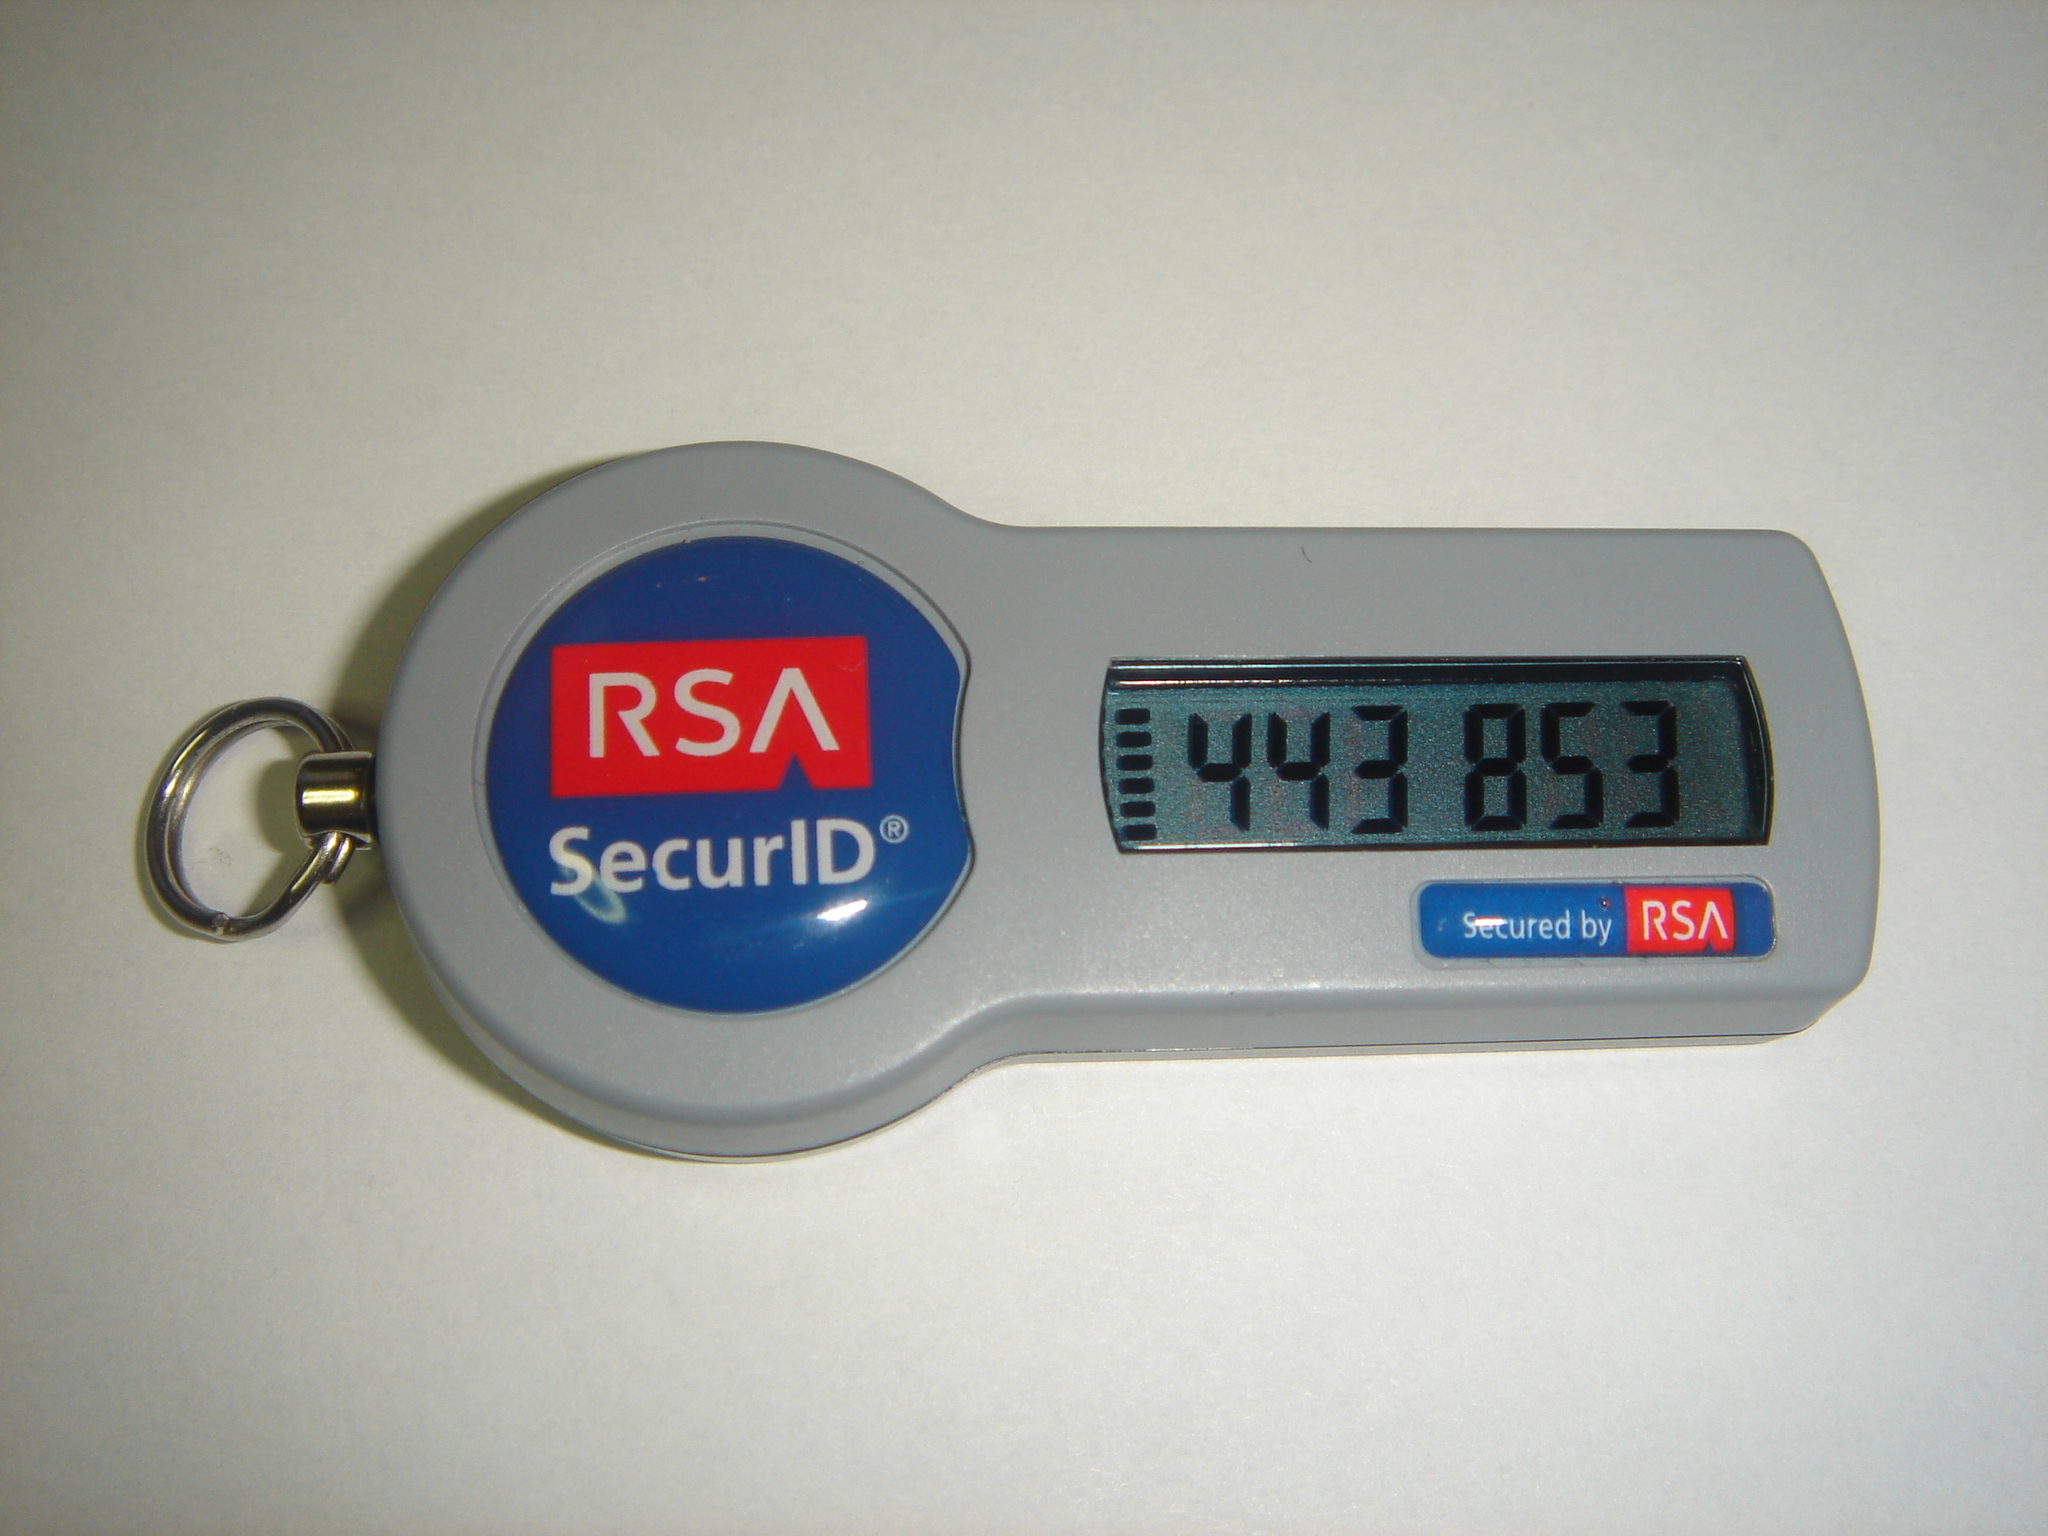
\includegraphics [width=7.5cm] {images/token_itau.jpg}
\caption{Token em formato de chaveiro} \label{fig_token_itau}
\end{center}
\end{figure}


Biometria � a ci�ncia de reconhecer a identidade de uma pessoa baseada em seus atributos f�sicos e/ou comportamentais, tais como a face, as impress�es digitais, veias da m�o, voz e a �ris \cite{li2011handbook}. O uso da biometria como fator de autentica��o possu� algumas vantagens. Naturalmente, n�o � poss�vel esquecer uma caracter�stica biom�trica e dificilmente esta caracter�stica desaparece repentinamente (talvez em casos de acidentes graves). Caracter�sticas biom�tricas s�o intr�nsecas a pessoa que as possui e portanto � intransfer�vel. Como desvantagem, a biometria pode variar drasticamente ao longo do tempo. Como exemplo, a voz humana pode variar repentinamente quando estamos doentes; nossos tra�os faciais infelizmente envelhecem ao longo do tempo. Vale ressaltar que m�todos de autentica��o baseados em biometr�a s�o probabil�sticos, ou seja, pode ser que o sistema de autentica��o rejeite uma entrada aut�ntica devido � uma s�rie de fatores externos.

As caracter�sticas humanas para serem utilizadas em uma m�todo de autentica��o biom�trica devem satisfazer alguns requisitos, dentre eles destacam-se:

\begin{itemize}
        \item Universalidade (toda pessoa deve possu�-la);
        \item Unicidade (deve permitir distinguir as pessoas);
        \item Estabilidade (n�o deve se alterar demasiadamente ao longo do tempo);
        \item Coletabilidade (deve poder ser medida quantitativamente);
        \item Desempenho (deve possibilitar um reconhecimento preciso, em tempo h�bil);
        \item Aceitabilidade (deve ser aceitos facilmente por seus usu�rios);
        \item Circunven��o (deve dificultar a possibilidade de fraudes).
\end{itemize}

A tabela \ref{tb:comparacao} apresenta um comparativo realizado por \cite{maltoni2009handbook} entre as caracter�sticas biom�tricas mais utilizadas. � poss�vel observar que nenhuma das biometr�as apresentadas consegue atender todos estes requisitos com excel�ncia e a escolha de qual utilizar deve levar em conta a natureza e as exig�ncias de cada aplica��o \cite{jain1999biometrics}.

\begin{table}[ht]
\caption{Compara��o das caracter�sticas biom�tricas mais utilizadas}
\begin{center}
    \begin{tabular}{ | c | c | c | c | c | c | c | c |}
    \hline
    \textbf{Caracter�stica} & \rotatebox{90}{\textbf{Universalidade}} & \rotatebox{90}{\textbf{Unicidade}} & \rotatebox{90}{\textbf{Estabiliade}} & \rotatebox{90}{\textbf{Coletabilidade}} & \rotatebox{90}{\textbf{Desempenho}} & \rotatebox{90}{\textbf{Aceitabilidade}} & \rotatebox{90}{\textbf{Circunven��o}} \\ \hline
    Face                             & Alta      & Baixa  & M�dia & Alta     & Baixa  & Alta      & Baixa \\ \hline
    Impress�o Digital      & M�dia  &  Alta    & Alta      & M�dia & Alta     & M�dia  & M�dia \\ \hline
   Geometria das m�os & M�dia  & M�dia & M�dia & Alta     & M�dia & M�dia  & M�dia \\ \hline
    Veias da m�o/dedo  & M�dia  & M�dia  & M�dia & M�dia & M�dia & M�dia & Alta \\ \hline
    �ris                                & Alta      & Alta       & Alta     & M�dia & Alta     & Baixa  & Alta \\ \hline
    Assinatura                  & Baixa   & Baixa   & Baixa  & Alta     & Baixa  & Alta     & Baixa \\ \hline
    Voz                              & M�dia  & Baixa   & Baixa  & M�dia & Baixa  & Alta     & Baixa \\ \hline
    \end{tabular}
\end{center}
\label{tb:comparacao}
\end{table}

Sistemas de autentica��o biom�trica podem ser grosseiramente representados segundo o fluxograma da Figura \ref{fig:diagram_attacks}.

\begin{figure}[!htb]
\begin{center}
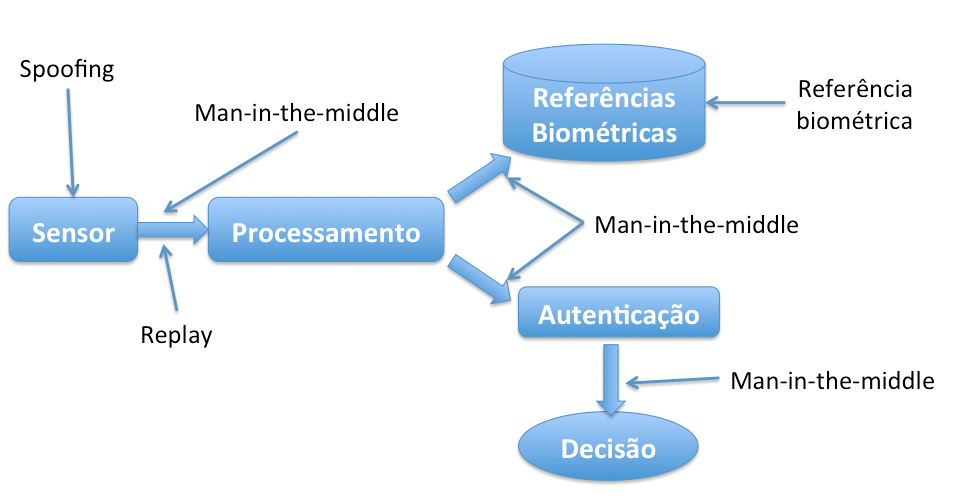
\includegraphics [width=13cm] {images/diagram_attacks.png}
\caption{Fluxograma de um sistema de autentica��o biom�trica} \label{fig_diagram}
\end{center}
\end{figure}

Primeiramente o trato biom�trico � capturado via algum tipo de \textbf{sensor}. Ap�s esta captura, o trato biom�trico capturado � \textbf{processado} a fim de extrair as caracter�sticas biom�tricas e gera��o da refer�ncia biom�trica. Quando se est� efetuando o cadastro de uma refer�ncia biom�trica, estas caracter�sticas s�o \textbf{armazenadas} em uma base de dados para acessos futuros. Quando se est� efetuando a \textbf{autentica��o}, estas caracter�sticas biom�tricas ser�o utilizadas no processo de compara��o com alguma identidade requerida no banco de dados. Conforme pode ser observado na  figura ataques podem ser efetuados em qualquer ponto da arquitetura \cite{xiao2005security}. As pr�ximas subse��es ir�o discorrer sobre cada um dos poss�veis ataques e solu��es para mitig�-los.

\subsection{Ataque de \textit{replay}}

O ataque de replay consiste da utiliza��o de dados previamente submetidos da identidade alvo para o sistema de autentica��o a fim de obter o acesso n�o autorizado. Estes dados podem ser obtidos interceptando (\textit{sniffing}) o canal de dados entre o sensor e a unidade de processamento de dados biom�tricos durante uma autentica��o bem sucedida da identidade alvo. Para deter ataques dessa natureza, o sistema de autentica��o biom�trica deve assegurar que o dado fornecido n�o foi injetado artificialmente. Uma forma de se defender deste tipo de ataque � fazer uso da caracter�stica probabil�stica da pr�pria biometria. � praticamente imposs�vel dois processos de captura independentes e em intervalos de tempo distintos gerar exatamente o mesmo dado biom�trico. Se isto ocorrer � prov�vel que este dado foi interceptado e est� sendo injetado no sistema de autentica��o \cite{xiao2005security}.

\subsection{Ataque na refer�ncia biom�trica}

O ataque de refer�ncias biom�tricas consiste em atacar o local de armazenamento das refer�ncias biom�tricas. Com este tipo de ataque pode-se: adicionar uma biometria falsa no sistema de armazenamento, copiar as refer�ncias biom�tricas armazenadas, remover alguma refer�ncia biom�trica ou modificar as refer�ncias biom�tricas existentes \cite{uludag2004attacks}. Dentre estas possibilidades a mais perigosa � a c�pia de refer�ncias biom�tricas, pois as mesmas podem ser usadas, atrav�s de engenharia reversa, para gerar biometrias falsas. \cite{hill2001risk} demonstrou que � poss�vel gerar impress�es digitais falsas atrav�s do processo de engenharia reversa com refer�ncias biom�tricas baseadas em min�cias. Com estas impress�es digitais fabricadas, foi poss�vel violar um sistema de autentica��o baseado em impress�es digitais. Um outro ponto de destaque neste tipo de ataque � que uma vez violada uma refer�ncia biom�trica, a mesma perde a caracter�stica da unicidade.

\subsection{Ataque \textit{man-in-the-midle}}

O ataque \textit{man-in-the-middle} ou homem do meio � uma forma de ataque em que os dados trocados entre os componentes do sistema de biometria s�o, de alguma forma, interceptados e alterados pelo atacante. Neste tipo de ataque o atacante pode: interceptar dados sensor, interceptar dados enviados para armazenamento e interceptar dados de decis�o do sistema de biometria. Mecanismos como encripta��o dos dados antes de serem transmitidos e/ou prover canais de comunica��o seguro podem mitigar este tipo de ataque.

\subsection{Ataque de spoofing}

O ataque de \textit{spoofing} em sistemas de autentica��o biom�trica, � um tipo de ataque em que o atacante forja o trato biom�trico alvo apresentando uma biometria falsa ao sensor, burlando o sistema de autentica��o. Em sistemas de autentica��o baseados em biometria h� duas motiva��es para se forjar um trato biom�trico. A \textbf{primeira} motiva��o � o atacante obter o trato biom�trico de outra pessoa a fim de tomar sua identidade. Em sistemas de autentica��o baseados na voz, o atacante pode gravar a voz da identidade alvo e usar esta grava��o como entrada no sistema de autentica��o. Em sistemas de autentica��o baseados em impress�es digitais o atacante pode obter alguma impress�o latente da identidade alvo e gerar um dedo artificial contento a impress�o digital roubada. A saber em \cite{uludag2004attacks}, \cite{leyden2002gummi} e \cite{matsumoto2002impact} s�o trabalhos relacionados a ataques de \textit{spoofing} em sistemas de autentica��o baseados em impress�es digitais, em \cite{johnson2010multimodal}, \cite{kanematsu2007highly} e \cite{pacut2006aliveness} s�o trabalhos relacionados a ataques de \textit{spoofing} baseados na biometria da iris e em \cite{chetty2004liveness} e \cite{eveno2005speaker} s�o trabalhos relacionados a ataques de \textit{spoofing} em sistemas de autentica��o baseados na biometria da voz humana. A \textbf{segunda} motiva��o � um atacante gerar um trato biom�trico totalmente artificial (sem se basear em uma biometria real), a fim de enganar o sistema de cadastro e autentica��o biom�tricos. Com isso, o atacante pode compartilhar esta biometria falsa com outros atacantes.

Melhores pr�ticas de seguran�a orientam utilizar mecanismos como, criptografia de dados e cria��o de canais seguros para mitigar ataques para a maioria dos casos citados anteriormente \cite{xiao2005security}. No caso dos ataques de \textit{spoofing}, o sensor de biometr�a (ponto alvo deste tipo de ataque) � o �nico ponto do fluxograma da Figura \ref{fig_diagram} em que nenhum dos mecanismos s�o efetivos para mitig�-los, tornando-se assim o ponto mais fr�gil a ataques.


%%%%%%%%
% Objetivos, Hip�teses e Resultados esperados
%%%%%%%%
\section{Objetivos, Hip�teses e Resultados esperados}


%%%%%%%%
% Organiza��o do trabalho
%%%%%%%%
\section{Organiza��o do trabalho}
\chapter{Revis�o da literatura}
\chapter{Metodologia}




\chapter{Resultados e conclus�es parciais}

\section{Resultados preliminares}

\begin{table*}[ht!]
\caption{$HTER(\%)$ of each countermeasure applying the intra-test ($D_1=D_2$) and the inter-test ($D_1 \neq D_2$) protocol.}
\begin{center}
  \begin{tabular}{ | c | c | c | c  c |  c  | }
    \hline

   \multirow{2}{*}{\textbf{Countermeasure}} & \textbf{Train/Tune} & \textbf{Test} & \multicolumn{2}{c|}{\textbf{HTER(\%)}} & \textbf{HTER degradation (test set) between}\\ 
     & EER in $D_1$ & $D_2$ & \textbf{dev} & \textbf{test}  & $D_1 = D_2$ and $D_1 \neq D_2$ \\ \hline
    
    \multirow{4}{*}{Correlation} & Replay  & Replay  &  11.66 & 11.79 & \multirow{2}{*}{$424.00\%$}\\ 
               &  \footnotesize{$EER=11.66\%$}& CASIA & 59.12 & 61.78  & \\ \cline{2-6}
               & CASIA  & Replay & 49.34 & 48.47  & \multirow{2}{*}{$54.56\%$}\\  
               & \footnotesize{$EER=24.91\%$}  & CASIA  & 24.91 & 31.36 & \\ \hline \hline

    \multirow{4}{*}{$LBPTOP_{8,8,8,1,1,1}^{u2}$}  & Replay & Replay  & 8.17 & 8.51  & \multirow{2}{*}{$499.88\%$} \\
               &  \footnotesize{$EER=8.17\%$}  & CASIA  & 52.32 & 51.05 &  \\ \cline{2-6}
               & CASIA  & Replay & 60.09 & 61.11  & \multirow{2}{*}{$174.40\%$} \\ 
               & \footnotesize{$EER=21.77\%$}   & CASIA  & 21.77 & 22.27 & \\ \hline \hline

    \multirow{4}{*}{$LBP_{8,1}^{u2}$} & Replay  & Replay  & 14.41 &15.45 & \multirow{2}{*}{$211.07\%$} \\
               &  \footnotesize{$EER=14.41\%$}  & CASIA  & 46.87  & 48.06  & \\ \cline{2-6}
               & CASIA  & Replay & 55.21 & 57.64  & \multirow{2}{*}{$155.72\%$} \\
               & \footnotesize{$EER=23.00\%$}  & CASIA  & 23.00  & 22.54 & \\
            
    \hline
  \end{tabular}
\end{center}
\label{tb:CrossTest}
\end{table*}


Analyzing the performance in the intra-test protocol ($D_1 = D_2$) it can be observed a good  performance and a good intra-database generalization power of the three evaluated countermeasures. Note that the countermeasure based on $LBP-TOP$ is the state-of-art in both databases \cite{Pereira_LBP_2012} and \cite{JukkaLBP2012}. The good generalization performance can be attested comparing the results between the development set and the test set. In Table \ref{tb:CrossTest} the $HTER(\%)$ in the development set and the $HTER(\%)$ in the test set are very similar. In Figure \ref{fig:ROC_cross} the ROC curves blue and red (dashed line and solid line) represents the intra-test test protocol. It can be observed that the curves are almost overlapped.





%=============================== Bibliografia ===============================================
\addcontentsline{toc}{chapter}{Bibliografia}
\renewcommand{\bibname}{Bibliografia}
\markboth{Bibliografia}{Bibliografia}

\bibliographystyle{dcu}
\bibliography{meubib}


\end{document}
